\documentclass[10pt]{article}
\makeindex
\usepackage{amsmath, amsfonts, amssymb, amstext, amscd, amsthm, graphicx,makeidx, hyperref, url, pgfplots, mathrsfs, mathtools}
\graphicspath{ {./images/} }
\pgfplotsset{width=7cm,compat=1.8}
\usepackage[margin=1.0in, headheight=40pt]{geometry}
\usepackage{fancyhdr}
\usepackage[english]{babel}
\usepackage[utf8]{inputenc}

\usepackage{caption}
\usepackage{subcaption}

\makeatletter
\renewcommand*\env@matrix[1][*\c@MaxMatrixCols c]{%
  \hskip -\arraycolsep
  \let\@ifnextchar\new@ifnextchar
  \array{#1}}
\makeatother

\allowdisplaybreaks
\newcommand{\R}{\mathbb{R}}
\newcommand{\C}{\mathbb{C}}
\newcommand{\Z}{\mathbb{Z}}
\newcommand{\N}{\mathbb{N}}
\newcommand{\Q}{\mathbb{Q}}
\newcommand{\F}{\mathbb{F}}
\newcommand{\ddx}{\frac{d}{dx}}

\pagestyle{fancy}
\fancyhf{}
\cfoot{\thepage}
\lhead{Alvin On\\
	  Nathan Suri\\
	  Laura Lewis
}
\chead{CS 101-3}
\rhead{Due Date: 6/6/2020}
\begin{document}
\begin{center}
\section*{Wave Function Collapse Project}
\end{center}

\section{Project Description}
We proposed our own project, based on the WaveFunctionCollapse algorithm, which can be seen \href{https://github.com/mxgmn/WaveFunctionCollapse}{here}. The original algorithm is a procedural generation algorithm to generate bitmaps that are locally similar to the input bitmap. The general idea is that based on this input bitmap, we are given a set of states (tiles) with neighboring constraints as input, where we want to randomly generate a larger board of a given size that satisfies the neighboring constraints from this. The original algorithm is based on quantum mechanics, where it initializes all tiles in a superposition of all states in the input and then observes the tile with the lowest entropy to collapse it. Following this, the changes caused by the collapse are propagated through the rest of the board until all constraints are satisfied. This repeats until all tiles are collapsed into a single state, in which we have the board we wanted to generate.\\
\indent Given this clear underlying quantum structure to the problem, our main goal was to incorporate our knowledge of quantum programming and algorithms from this course into the project, replacing certain parts of the algorithm with quantum ideas rather than this classical simulation of it. We aimed to do so in two different ways.\\
\indent The first was to keep the mainly classical approach to the algorithm and analyze the effect of utilizing a quantum random number generator to select the state for collapse. In the original algorithm, this state is selected using numpy's random.choice function. However, we were interested in seeing what difference, if any, it would make to adjust this to use a quantum random number generator. Furthermore, this was the first step in allowing us to begin incorporating more quantum ideas into the algorithm. To implement this, we did so in Q$\#$, where we generated a single random bit by applying the Hadamard gate to a qubit in the zero state. This causes the qubit to be in an equal superposition, such that upon measuring in the computational basis, we obtain a completely random result. Thus, we then obtained a random bit string by concatening many of these random bits, which we converted into an integer to obtain our final random integer to pass to the classical program. Furthermore, the classical program itself is largely a Python version of the original algorithm, which we will discuss in the Implementation section.\\
\indent Our second method for incorporating quantum computation into the WaveFunctionCollapse algorithm was through an algorithm similar to VQE from lecture. From our input image, we obtain frequencies for the tiles. Then, using the encodeInput operation from HW 4 Task 4A, we can obtain a superposition with these frequencies as the amplitudes. Furthermore, by using a variational approach, we can then arrive at the correct entanglement scheme in order to arrive at a board where the constraints are satisfied. This involves a quantum and classical hybrid algorithm very similar to VQE. Our idea for this was to have a parameterized quantum circuit, which takes in our parameters and the tiles in superposition, and strongly entangles the neighboring qubits. In analogy with VQE, this circuit has layers of single and two-qubit gates, where the two-qubit gates in this case only need to act on neighboring qubits, as the constraints for the board are only local. After applying this circuit to the tiles in superposition, we measure the qubits and pass the results to the classical machine in its loss function. The loss is then calculated by penalizing any configuration where the constraints are not satisfied. Finally, we iterate and update the parameters of the circuit based on the loss function until we have a state which satisfies our constraints, which is the board we need.

\section{Implementation}
\section{Results}
After testing on several input images, a sample of the results we obtained are below. We only included the Red Maze and Bricks input images as tests for the sake of space in this report. First, in Figure 1, the original input patterns for the Red Maze and Brick patterns are shown. Following this, in Figures 2 and 3, we display different results from the completely classical WaveFunctionCollapse algorithm implemented in Python versus the WaveFunctionCollapse algorithm with quantum random number generation included when we choose which state we want to collapse. Obviously, these results will be slightly difference due to the randomness in each of them, but the result overall is still what we expected, in that the output images are both locally similar to their respective inputs. 
\newpage
\begin{figure}[h]
\centering
\begin{subfigure}{.5\textwidth}
  \centering
  
\includegraphics[scale=5]{RedMaze}
  \caption{Red Maze Original Pattern}
\end{subfigure}%
\begin{subfigure}{.5\textwidth}
  \centering
  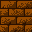
\includegraphics[scale=1]{3Bricks}
  \caption{Bricks Original Pattern}
\end{subfigure}
\caption{Original Input Patterns}
\label{fig:test}
\end{figure}

\begin{figure}[h]
\centering
\begin{subfigure}{.5\textwidth}
  \centering
  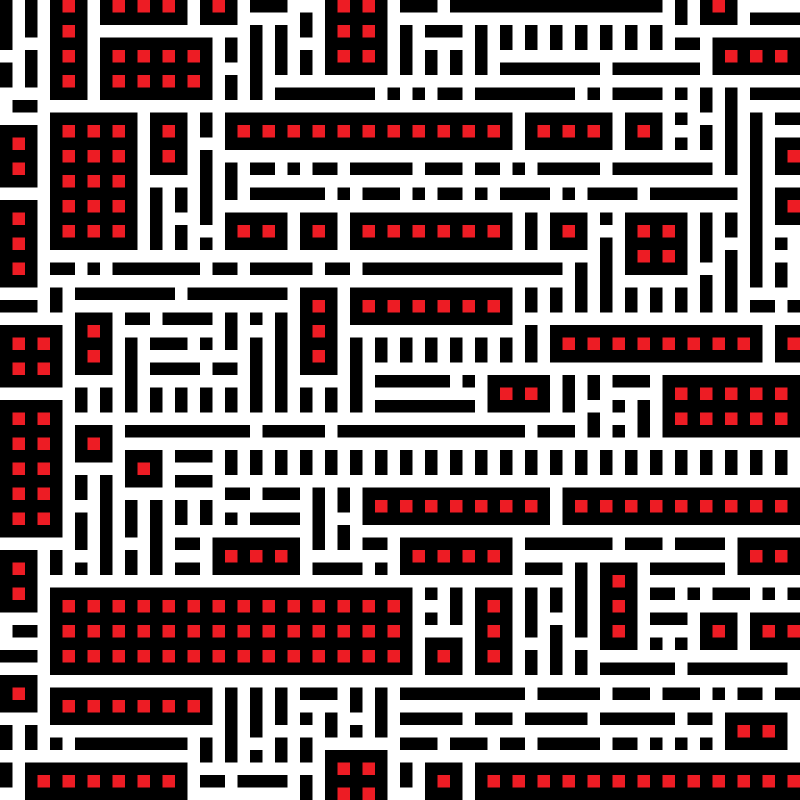
\includegraphics[scale=0.22]{redResultQRNG}
  \caption{Wave Function Collapse with QRNG}
  \label{fig:sub1}
\end{subfigure}%
\begin{subfigure}{.5\textwidth}
  \centering
  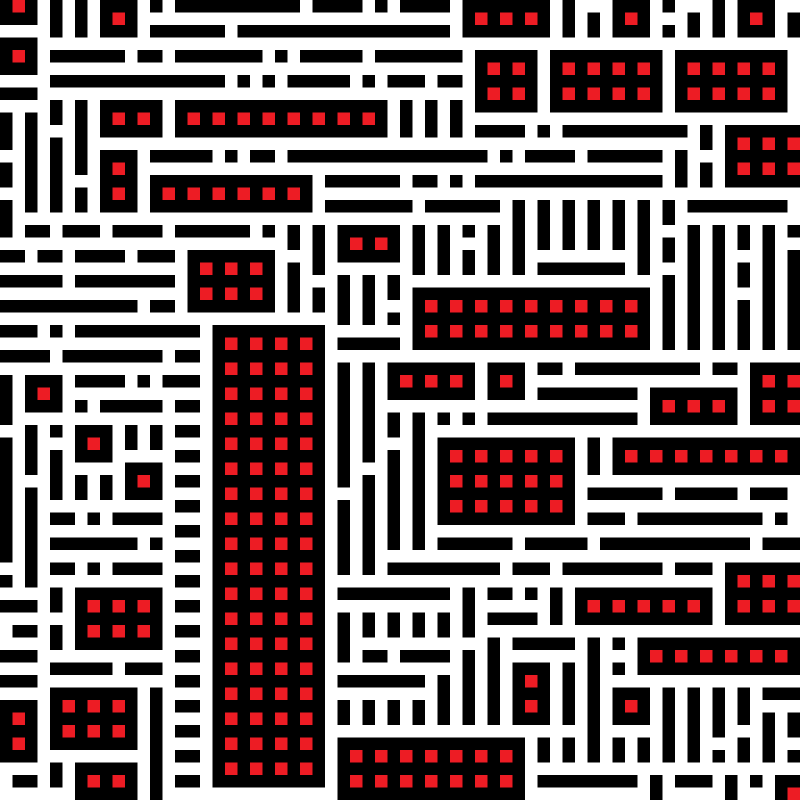
\includegraphics[scale=0.22]{redResultClassical}
  \caption{Classical Wave Function Collapse}
  \label{fig:sub2}
\end{subfigure}
\caption{Comparison of Classical and QRNG Wave Function Collapse for Red Maze Pattern}
\label{fig:test}
\end{figure}
\begin{figure}[h]
\centering
\begin{subfigure}{.5\textwidth}
  \centering
  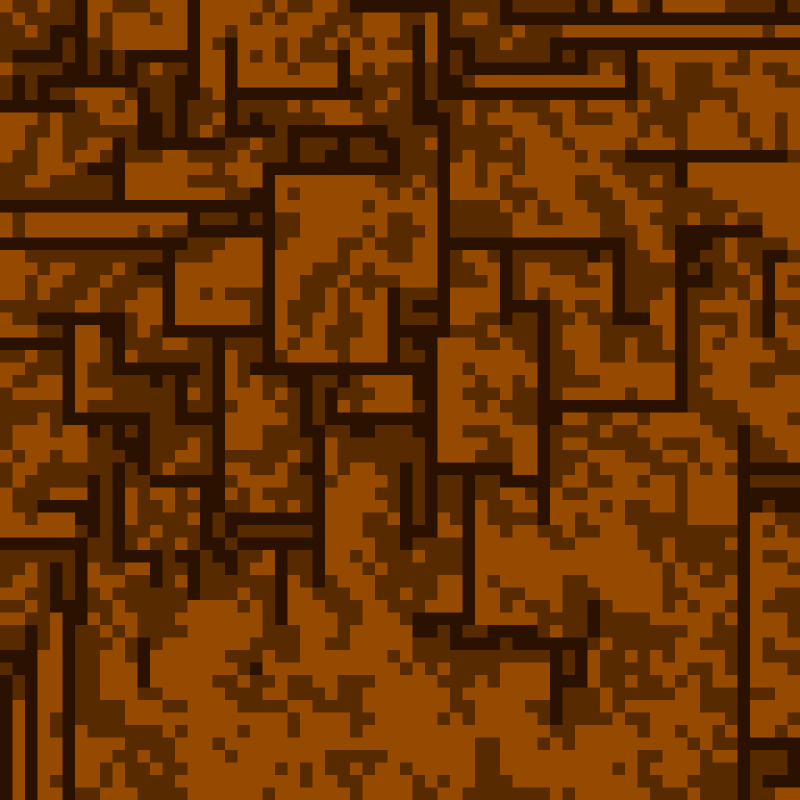
\includegraphics[scale=0.2]{bricksResultQRNG}
  \caption{Wave Function Collapse with QRNG}
  \label{fig:sub1}
\end{subfigure}%
\begin{subfigure}{.5\textwidth}
  \centering
  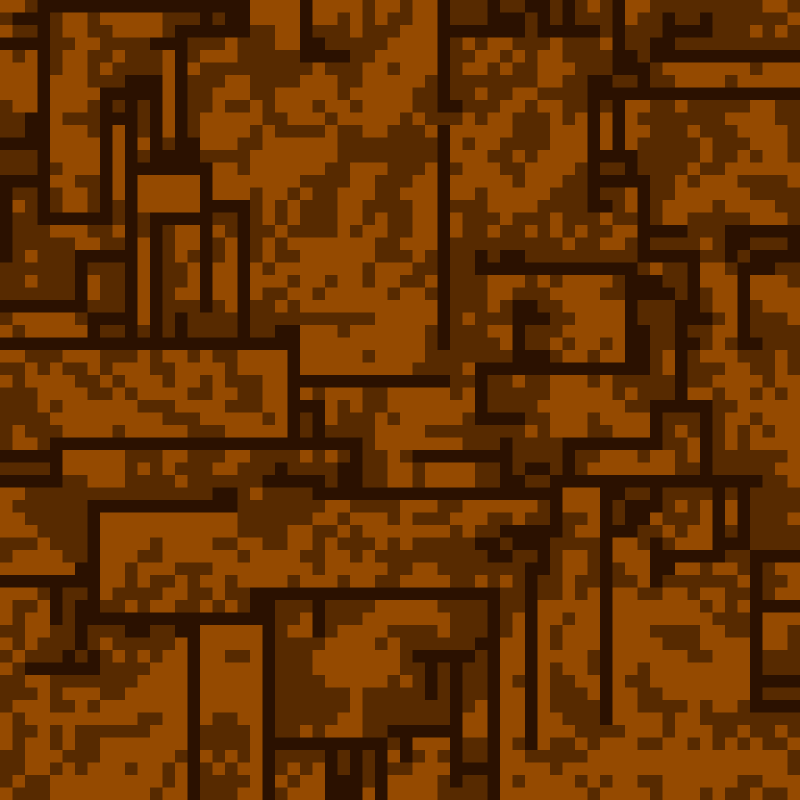
\includegraphics[scale=0.2]{bricksResultClassical}
  \caption{Classical Wave Function Collapse}
  \label{fig:sub2}
\end{subfigure}
\caption{Comparison of Classical and QRNG Wave Function Collapse for Brick Pattern}
\label{fig:test}
\end{figure}

\newpage
\section{Tests}
The tests we considered were based off of input images provided in the original implementation of the WaveFunctionCollapse algorithm. Given these input images, we can output what our board generated and observe whether or not this output image is locally similar to the original input. The input images are small and indicate which pattern we expect to see in the much larger output image. We considered in total eight input images to test this on.

\end{document}